
%************************************************
\chapter{Introduction}\label{ch:introduction}

%************************************************
\section{Array CGH}
Array \ac{CGH} is a commonly used diagnostic test in clinical genetics. The test utilises many probes (from 44,000 to 1,000,000) affixed to a glass slide. 
Each probe consists of many copies of an oligonucleotide 40-60 base pairs long, designed to target a specific region of the genome. Two samples are hybridised to the array in a competitive reaction, usually a diagnostic sample in competition with a reference sample. 
\paragraph*{}
The diagnostic and reference samples are labelled with a fluorescent dye (patient \ac{Cy5} and reference \ac{Cy3}). Once hybridised the array is scanned, capturing the excitation of each dye, producing a high resolution image of the array \cite{ahn2010}. This image undergoes feature extraction to calculate the Cy5 and Cy3 signal intensities at each probe and associated quality scores.
\paragraph*{}
This data can then be analysed for copy number variation by applying one of a number of available algorithms: Probe scores are normalised, split into segments of equal copy number and each segment assigned a copy number status \cite{hupe2004}.
\paragraph*{}
Dividing the signal intensity of Cy5 by that of Cy3 produces a ratio where equal copy number is 1. This ratio is then logged (base 2) to produce the log2 ratio where equal copy number is 0, a decrease in copy number is indicated by a negative value and increased copy number a positive  value. 
\section{Copy Number Variation (CNV)}
\ac{CNV} is a deviation in copy number from a reference genome which typically contains 2 copies of a DNA segment \cite{roy2013}. CNV can occur in recombination and replication events. CNV can be benign polymorphisms or associated with Mendelian, sporadic and complex disease possibly through gene dosage, disruption, fusion or positional effects \cite{zhang2009}.
\section{Application of array CGH in clinical setting}
In 2009, array CGH started replacing karyotyping as the method for detection of CNV in NHS diagnostic genetic services. Array CGH offers a higher resolution, less reliance on analyst interpretation/skill and the advantage of a high throughput practical workflow, however few Trusts actually have this test commissioned as a first line test due to the higher cost. Guy`s and St Thomas` NHS Trust adopted a patient to patient hybridisation approach, halving the cost of consumables by replacing the reference sample with another patient sample \cite{ahn2010}.

\paragraph*{}
The product of the increased resolution of arrays is a higher abnormality pick up rate than karyotyping (25\% vs 3.7\%) \cite{ahn2013,jordan_microarrays_2012}. 

\section{Patient to patient hybridisation}
As array CGH compares two samples, the use of a reference sample infers any CNV detected is from the patient. Hybridising two patients removes this assumption, producing two challenges:
\begin{enumerate}
\item Is a CNV a duplication in one patient, or a deletion in the second patient?
\item If both patients have the same CNV relatively no difference would be seen, resulting in a `normal` log ratio so the CNV would not be detected.
\end{enumerate}
\begin{figure}
\centering
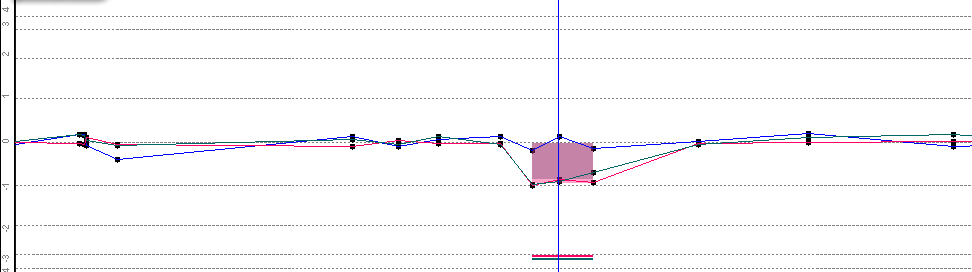
\includegraphics[width=\linewidth]{./Figures/SharedImbalance.jpg}
\caption[A trace showing how a shared imbalance would not be detected]{Three array traces are shown. Two arrays (Red and green traces) have the same three probe deletion on chromosome 6. The dark blue trace shows the two arrays hybridised together insilico. The log ratio appears completely normal and the deletion is not detected.}
\label{fig:SharedImbalance}
\end{figure}

\paragraph*{}
The first challenge can be overcome by comparing the signal intensities of each dye across the CNV and normal regions. The sample where the signal intensities within the CNV are markedly different from the normal regions contains the CNV.

\paragraph*{}
The second challenge is currently overcome with ``a careful consideration of patient referral information`` to reduce the risk of this occurring. Hybridisation partners are mismatched on phenotype \cite{ahn2010}. This assumes that patients with differing referral reasons eg heart vs renal defects will not have the same underlying CNV. Furthermore, CNV is rare and therefore the risk of two patients with the same CNV being hybridised together is low to start with, even without phenotype mismatching.

\section{Project Rationale}
Financial pressures on the NHS are requiring increasingly innovative approaches. Adopting a patient to patient hybridisation approach halves the cost of performing the test \cite{ahn2010}.
\paragraph*{}
One fear preventing adoption of a patient to patient approach in a clinical setting is the fear of missing a diagnosis due to shared CNV in hybridisation partners \cite{dunlop2015}. 
\paragraph*{}
In a clinical setting it is important to have a high test sensitivity and specificity. Any missed diagnoses due to the patient to patient approach would be a false negative, a type two error, reducing the sensitivity of the test.  A test must have a high specificity where as a screen can afford to have a higher level of false positives if followed by a test.
\paragraph*{}
A false negative misses a chance of diagnosis, extending the patient`s diagnostic odyssey, or may result in a normal report incorrectly being issued for a prenatal test, potentially resulting in an affected child. 
\paragraph*{}
The chance of two patients having the same aberration (without phenotype mismatching) has been calculated as 1 in 6000 \cite{joowook_ahn_frequency_2015}.
\paragraph*{}
Whilst the chance of this occurring is low, and is mediated with strategies such as mismatched phenotypes, with 4000 arrays performed each year this could occur every 1.5 years (without phenotype mismatching). 
\paragraph*{}
An array run starts with the creation of a worksheet. This worksheet defines which patients will be hybridisation partners.  Hybridisation partners must be phenotype mismatched, a process performed by one clinical scientist and checked by a second. For a run of 96 samples worksheet creation and checking can take three hours.
The efficacy can be affected by incorrect, limited or vague phenotype information.
\paragraph*{}
Simplifying the creation of a worksheet will save time, possibly reassigned to a lower grade staff member and may also be automatable, further reducing the cost of processing an array.
\paragraph*{}
More importantly further reducing the chance of missing an CNV improves the service the patient receives, ending, or preventing a diagnostic odyssey.

\section{Project Aims}
The aim of this project is investigate a tool which is run during data processing and acts as a screen to detect CNV before the array present in both hybridisation partners.

\section{Array Design}
The arrays, reagents, equipment and software used to process and analyse are manufactured by Agilent Technologies \cite{agilenttechnologies_microarrays}.
\paragraph*{}
The array is an 8x60K array with a median resolution of 120kb. 
\paragraph*{}
The array was custom designed using the online probe catalogue eArray \cite{agilenttechnologies_earray}. The array design consists of 46554 probes. 3886 are control probes and 42658 are targeted of which 29 are duplicated leaving 42629 unique probes.
\paragraph*{}
A request for a tool similar to the aims of this project was sent to and declined by Agilent.

\subsection{Feature Extraction}
After the arrays have been processed in the laboratory and scanned (Figure \ref{fig:microarrayslide}) the array image undergoes feature extraction.
\begin{figure}
\centering
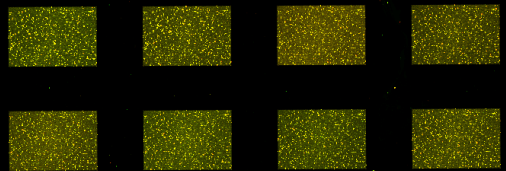
\includegraphics[width=\linewidth]{./Figures/microarrayslide}
\caption[A scanned 8 x 60k array]{A scanned array slide containing 8 arrays}
\label{fig:microarrayslide}
\end{figure}

\paragraph*{}
The feature extraction software converts the raw signal image into measurements for each probe. At each probe the excitation of each dye is captured as the signal intensity. This intensity is processed, including a normalisation step across all probes producing a processed signal intensity normalised to 1000 \ac{AFU}.
\paragraph*{}
At each probe a log ratio is calculated from the two signal intensities (equation \ref{eq:logratio})
\begin{equation}\label{eq:logratio}
Log10\ \frac{Cy5\ signal\ intensity}{Cy3\ signal\ intensity}
\end{equation} 

\subsection{Feature Extraction File}
The result of feature extraction is one feature extraction file per array, a tab delimited text file of 10-15mb in size.
\paragraph*{}
The feature extraction file can be created in four levels of  verbosity: full, compact (default), QC and minimal. 
\paragraph*{}
Each feature extraction file consists of three sections, the parameters, stats and features.  

\subsubsection{Parameters}
The parameters section contains 38 fields covering information relevant to all 8 arrays on the slide such as the scanner make and model, time, date and protocols or parameters used to scan the slide. 

\subsubsection{Stats}
The stats section  contains 189 fields covering array specific measurements, such as average intensities and the derivative log ratio spread (DLRS) which is an indicator of quality used during analysis.

\subsubsection{Features}
The majority of the file is made up by the features section with one row per probe consisting of 42 fields. 9 fields are identifiers such as the probe catalogue name, the genomic locations and flags to identify probes used as controls. The remaining 33 fields include the raw signal intensity measurement for Cy3 and Cy5 dyes, the log ratio, background signal intensities and flags to mark a probe as having an extreme signal intensity, saturated or non-uniform.

\section{Use of algorithms to detect copy number variation}
If all goals of this project are met the tool produced will have much the same role as the aberration detection algorithms, taking raw signal intensities and identifying CNV.
\paragraph*{}
There are a number of algorithms which call \ac{CNV} from \ac{CGH} data. These algorithms are recursive binary segmentation methods which break chromosomes into segments of equal copy number. Examples include Z scores, \ac{CBS}, \ac{ADM2}, Nexus and \ac{HMM}. 

\subsection{Z score algorithm}
A Z score is a statistical measure of deviation from the mean for a normally distributed population. The Z score algorithm assigns each probe a Z score based on the log ratio. Any probes outside a user defined cut off (R) are classified as an outlier, or significantly away from mean. 
\paragraph*{}
The number of probes classified as above (R) and below (R`) this threshold and total number of measurements (N) are recorded across small windows of the genome. 
\paragraph*{}
These `windows` can be specified as a number of adjacent measurements or a fixed size eg every 1MB. Within each window the abundance of probes which log ratios which deviate from the mean is measured (r:r`).
\paragraph*{}
A Z score is then calculated measuring the significance of the over-abundance of probes with a deviant score in this window \cite{agilent_technologies_agilent_2011}.

\subsection{Aberration Detection Method (ADM-1/ADM-2)}
These algorithms are designed by Agilent\cite{agilent_technologies_agilent_2011}. These algorithms do not used fixed windows but segment the genome into intervals of equal copy number using log ratio scores from adjacent probes to best define interval breakpoints.

\subsubsection{ADM-1}
Firstly the data is normalised by subtracting the mean log ratio and dividing by the variance, creating a normally distributed population with a mean of 0. 
\paragraph*{}
Each chromosome is then broken into intervals of equal copy number and intervals are assigned a score (S(I)) which denotes the difference from the mean. A user defined threshold is set and any intervals which are above this are called as an aberration.
\paragraph*{}
The interval with the highest score is selected and the same process is performed on this segment to further define breakpoints. This is repeated for all intervals with an S(I) above the threshold.
\subsubsection{ADM-2}
The ADM-2 algorithm builds on ADM-1 by including probe quality information to weight probe signal log ratios when assigning S(I).

\subsection{Circular binary segmentation (CBS)}
\ac{CBS} uses log ratios from adjacent probes to create intervals which, as opposed to ADM-1/2 (which classifies segments as aberrant or not), are grouped into intervals with equal copy number \cite{venkatraman2007}. 
\paragraph*{}
\begin{figure}[h]
\centering
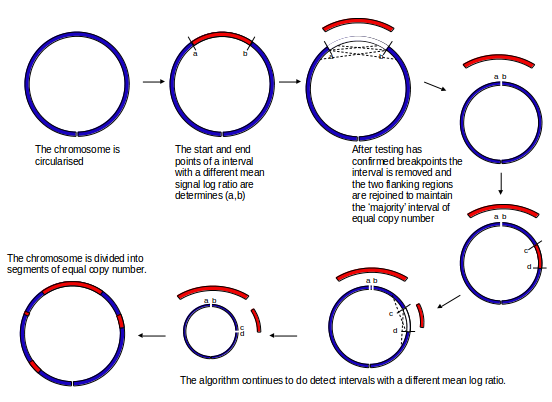
\includegraphics[width=1\linewidth]{./Figures/CBS}
\caption{Circular binary segmentation algorithm}
\label{fig:CBS}
\end{figure}

Each chromosome is made into a circle (Figure \ref{fig:CBS}). This allows for two break points to be identified, increasing the resolution of detection. When two breakpoints are detected the interval of potential different copy number is removed, and the flanking regions are joined to form a new circle. This allows a t-test to be performed between the mean log ratios on each interval. 
\paragraph*{}
Definition of an interval is determined using permutation testing, creating intervals using various breakpoints and looking for the most significant P value. If this P value is above a threshold an interval is created and the process is repeated for all intervals until no more changes are found.
\paragraph*{}
A number of checks are performed to ensure the correct end points have been found including edge effect correction, change point pruning and estimation of the log score distribution.

\subsection{Hidden Markov Model}
The hidden Markov model (HMM) \cite{agilent_technologies_agilent_2011} uses observations (log ratios) to determine the state of a hidden or latent value (copy number). The HMM has a chain property which takes into account the state of the previous probe.
\paragraph*{}
Firstly the data is segmented: the Haar wavelet is used to normalise the data before breakpoints are defined using preset parameters (FDR threshold). This step also calculates probabilities and probability distribution parameters used in later steps.
\paragraph*{}
The HMM is then applied. The forward-backward algorithm is used to calculate the posterior probabilities of the states. Baum-Welch learning uses these to ensure that each state has a well defined value.
\paragraph*{}
Finally the Viterbi algorithm is used to assign a state to each probe.

\subsection{Algorithm Performance}
Each algorithm performs differently depending on the signal:noise ratio and the size of the aberration\cite{willenbrock2005}.
\paragraph*{}
Circular binary segmentation (CBS) is rated as one of the most consistent performers albeit one of the most computationally demanding \cite{lai2005,willenbrock2005}. Some algorithms` performance varies greatly depending on user defined parameters which may be difficult to establish \cite{lai2005}.
\paragraph*{}
The algorithms described above are global segmentation methods which compare segments to the whole genome. Recently local segmentation methods have been described which look for CNV using high resolution data sets \cite{niu_screening_2012}. These algorithms have higher power than global algorithms but are less robust so an approach utilising both types of algorithm may produce the best performance \cite{roy2013}.

\section{Data storage and manipulation}
The tool requires data to be stored, curated and accessed. A database is an efficient tool for this role. 

\subsection{Relational database}
A relational database is a collection of tables where each row is an instance and each column is an attribute. Tables can be linked to store data in a simple and efficient manner.
\paragraph*{}
Relational databases are stored in a \ac{RDBMS} server such as MySQL or MS-SQL which can be installed locally or on a server to allow access from remote machines. A \ac{GUI} or `front end` enables user interaction with the data, commonly seen in Microsoft Access or an internet browser. 
\paragraph*{}
Database design and data manipulation/retrieval utilises the \ac{SQL}. 

\subsection{Non-relational database}
MongoDB \cite{mongodb_inc._mongodb_????} is an alternative database format to relational databases, storing data in BSON format, a binary form of the JSON format. JSON stores data as nested key-value pairs. 
\paragraph*{}
MongoDB does not require relationships between tables and fields to be defined, removing the need for complex joins and enables documents with differing formats to be easily stored and compared. MongoDB is faster and easier to scale than relational databases.

\subsection{Python}
Python is an object orientated programming language. Python programs can be written to perform a wide range of functions, such as parsing text files, performing complex mathematical and statistical calculations utilising additional modules or packages such as NumPy \cite{vanderwalt2011} and SciPy \cite{scipy_scipyorg_????}.
\paragraph*{}
Connectors are available (including MySQLdb \cite{dustman2014}, SQLAlchemy \cite{bayer_sqlalchemy_????}, PyODBC \cite{pyodbc_mkleehammer/pyodbc_????} and PyMongo \cite{pymongo_python_????}) enabling Python to interrogate and interact with databases.

\subsection{R statistical software package}
The R statistical software package \cite{rfoundationforstatisticalcomputing2014} has a repository of packages (Bioconductor \cite{huber_orchestrating_2015}) which includes packages which implement CNV algorithms such as \ac{CBS} within DNAcopy \cite{Sechan2015}.  